\documentclass[12pt,a4paper]{article}
% \usepackage{ctex}
\usepackage{amsmath,amscd,amsbsy,amssymb,latexsym,url,bm,amsthm}
\usepackage{epsfig,graphicx,subfigure}
\usepackage{enumitem,balance}
\usepackage{wrapfig}
\usepackage{mathrsfs,euscript}
\usepackage[usenames]{xcolor}
\usepackage{hyperref}
\usepackage[vlined,ruled,linesnumbered]{algorithm2e}
\usepackage{array}
\hypersetup{colorlinks=true,linkcolor=black}

\newtheorem{theorem}{Theorem}
\newtheorem{lemma}[theorem]{Lemma}
\newtheorem{proposition}[theorem]{Proposition}
\newtheorem{corollary}[theorem]{Corollary}
\newtheorem{exercise}{Exercise}
\newtheorem*{solution}{Solution}
\newtheorem{definition}{Definition}
\theoremstyle{definition}

\renewcommand{\thefootnote}{\fnsymbol{footnote}}

\newcommand{\postscript}[2]
 {\setlength{\epsfxsize}{#2\hsize}
  \centerline{\epsfbox{#1}}}

\renewcommand{\baselinestretch}{1.0}

\setlength{\oddsidemargin}{-0.365in}
\setlength{\evensidemargin}{-0.365in}
\setlength{\topmargin}{-0.3in}
\setlength{\headheight}{0in}
\setlength{\headsep}{0in}
\setlength{\textheight}{10.1in}
\setlength{\textwidth}{7in}
\makeatletter \renewenvironment{proof}[1][Proof] {\par\pushQED{\qed}\normalfont\topsep6\p@\@plus6\p@\relax\trivlist\item[\hskip\labelsep\bfseries#1\@addpunct{.}]\ignorespaces}{\popQED\endtrivlist\@endpefalse} \makeatother
\makeatletter
\renewenvironment{solution}[1][Solution] {\par\pushQED{\qed}\normalfont\topsep6\p@\@plus6\p@\relax\trivlist\item[\hskip\labelsep\bfseries#1\@addpunct{.}]\ignorespaces}{\popQED\endtrivlist\@endpefalse} \makeatother

\begin{document}
\noindent

%========================================================================
\noindent\framebox[\linewidth]{\shortstack[c]{
\Large{\textbf{Lab07-Amortized Analysis}}\vspace{1mm}\\
CS214-Algorithm and Complexity, Xiaofeng Gao \& Lei Wang, Spring 2021.}}
\begin{center}
\footnotesize{\color{red}$*$ If there is any problem, please contact TA Yihao Xie. }

\footnotesize{\color{blue}$*$ Name: WendiChen  \quad Student ID: 519021910071 \quad Email: chenwendi-andy@sjtu.edu.cn}
\end{center}
\begin{enumerate}
	\item Suppose we perform a sequence of n operations on a data structure in which the $i$ th 		operation costs $i$ if $i$ is an exact power of 2, and 1 otherwise. Use an accounting method to determine the amortized cost per operation.
	
	\begin{solution}
	~\\
	For the $i$-th ($2^k\le i < 2^{k+1},k\ge 0$) operation, an amortized cost $\widehat{C}_i$ = \$3 is charged. \$1 pays for the operation itself. \$2 is stored for the $2^{k+1}$-th operation.
	
    \begin{table}[htbp]
      \centering
      \caption{Table for Accounting Technique}
        \begin{tabular}{ccccccccccccc}
        i     & 1     & 2     & 3     & 4     & 5     & 6     & 7     & 8     & 9     & 10    & 11    & 12 \\
        $C_i$    & 1     & 2     & 1     & 4     & 1     & 1     & 1     & 8     & 1     & 1     & 1     & 1 \\
        $\widehat{C}_i$    & 3     & 3     & 3     & 3     & 3     & 3     & 3     & 3     & 3     & 3     & 3     & 3 \\
        Credit & 2     & 3     & 5     & 4     & 6     & 8     & 10    & 5     & 7     & 9     & 11    & 13 \\
        \end{tabular}%
      \label{tab:accounting}%
    \end{table}%
    
    We can find that the credit never goes negative. In other words, the sum of amortized cost provides an upper bound of the sum of actual costs.
    
    \begin{equation*}
        T(n) = \sum_{i=1}^{n}C_i \le \sum_{i=1}^{n}\widehat{C}_i=3n
    \end{equation*}
    
    Thus, the amortized cost per operation is $O(n)/n=O(1)$.
	\end{solution}

	\item Consider an ordinary \textbf{binary min-heap} data structure with $n$ elements supporting
the instructions \textsc{Insert} and \textsc{Extract-Min} in $O(\log n)$ worst-case time. Give a
potential function $\Phi$ such that the amortized cost of \textsc{Insert} is $O(\log n)$ and the
amortized cost of \textsc{Extract-Min} is $O(1)$, and show that it works.

    \begin{solution}
    ~\\
    Suppose the instructions \textsc{Insert} and \textsc{Extract-Min} cost $a\log n + c$ and $b\log n +d $ in worst-case time respectively. Define a potential function $\Phi = \sum_{i=1}^n b\log i$, where $n$ is the  size of the min-heap. The correctness is obvious because the potential is 0 for an empty min-heap and $\Phi$ never goes negative.\\
    For \textsc{Insert}, the amortized cost is
    \begin{align*}
        \widehat{C}_i &= C_i + \Phi_i - \Phi_{i-1}\\
        &\le a\log(i)+c+\log(i)\\
        &= O(\log i)\\
        &= O(\log n)
    \end{align*}
    For \textsc{Extract-Min}, the amortized cost is
    \begin{align*}
        \widehat{D}_i &= D_i + \Phi_{i} - \Phi_{i-1}\\
        &\le b\log(i)+d-b\log(i)\\
        &= O(1)
    \end{align*}
    Thus, the amortized cost of \textsc{Insert} and \textsc{Extract-Min} is $O(n\log n)/n=O(\log n)$ and $O(n)/n = O(1)$ respectively. 
    \end{solution}
	
	\item Assume we have a set of arrays $A_0, A_1, A_2,\cdots$, where the $i^{th}$ array $A_i$ has a length of $2^i$. Whenever an element is inserted into the arrays, we always intend to insert it into $A_0$. If $A_0$ is full then we pop the element in $A_0$ off and insert it with the new element into $A_{1}$. (Thus, if $A_{i}$ is already full, we recursively pop all its members off and insert them with the elements popped from $A_0,...,A_{i-1}$ and the new element into $A_{i+1}$ until we find an empty array to store the elements.) An illustrative example is shown in Figure \ref{Fig-MultiArray}. Inserting or popping an element take $O(1)$ time.

	\begin{figure}[!htbp]
	\centering
	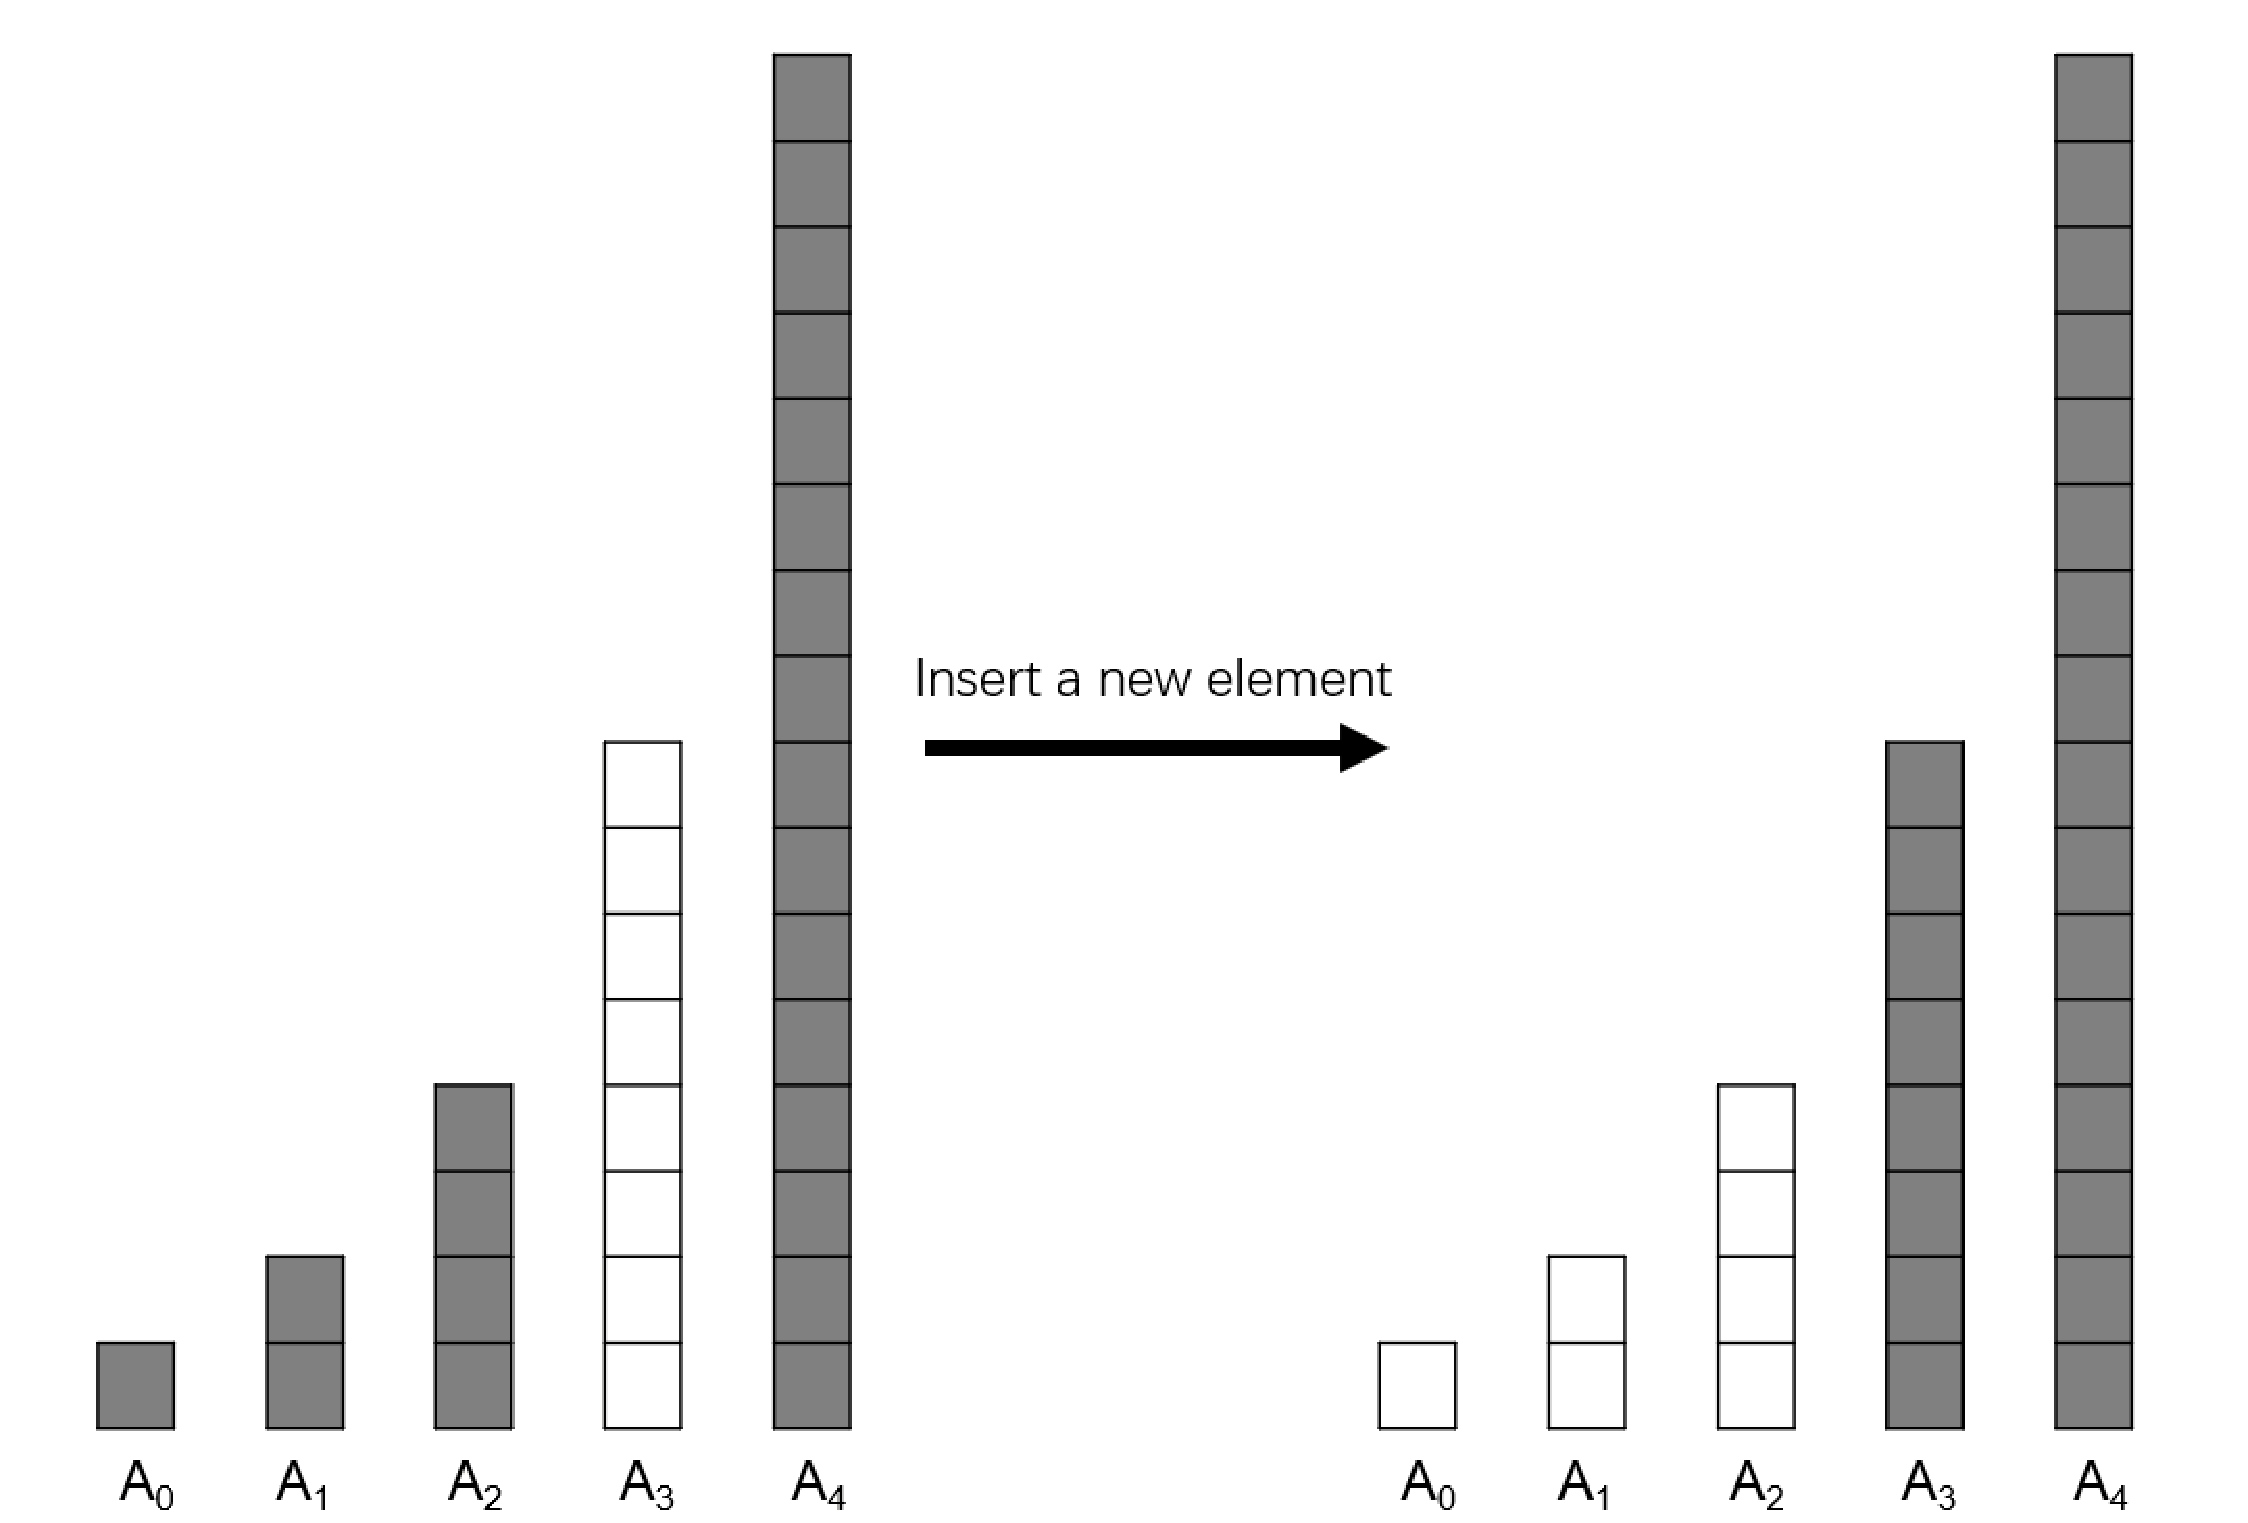
\includegraphics[width=0.5\textwidth]{Fig-MultiArray.pdf}
	\caption{An example of making room for one new element in the set of arrays.}
	\label{Fig-MultiArray}
	\end{figure}

    \begin{enumerate}
        \item In the worst case, how long does it take to add a new element into the set of arrays containing $n$ elements?
        \item Prove that the amortized cost of adding an element is $O(\log n)$ by \emph{Aggregation Analysis}.
        \item If each array $A_i$ is required to be sorted but elements in different arrays have no relationship with each other, how long does it take in the worst case to search an element in the arrays containing $n$ elements? 
\item What is the amortized cost of adding an element in the case of (c) if the comparison between two elements also takes $O(1)$ time?
    \end{enumerate}
    
    \begin{solution}
    ~
    \begin{enumerate}
        \item 
        In the worst case, we have to pop all the $n$ elements off and insert $n+1$ elements into an empty array. We have to do at most $2n+1$ operations. Thus, the time complexity in the worst case is $O(n)$.
        \item
        The scenario is similar to the case of incrementing a binary counter. What is different is that every flip in the $i$-position (which means we have to move all the elements to $i$-th array) has a cost of $2^i$. Thus, we can apply the aggregate technique. We assume $n = 2^k,k\ge 0$.
        \begin{align*}
            T(n) &= \sum_{i=1}^{n} C_i\\
            &= n \times 2^0+\frac{n}{2} \times 2^1 + \frac{n}{2^2}\times  2^2 + \dots \frac{n}{2^k}\times 2^k \\
            &=(k+1)n\\
            &=n(\log n + 1)
        \end{align*}
        Therefore, the amortized cost of adding an element is $O(n\log n)/n = O(\log n)$.
        \item
        In the worst case, we have to search every array, and for each array we have to search $\log(|A_i|)+1 = i+1$ times. For $n$ elements, we assume $n = 2^k-1,k\ge 1$. Then there will be $k$ arrays. The total number of operations (or time complexity) can be calculated by
        \begin{align*}
            \sum_{i=1}^{k} i = \frac{k(k+1)}{2} = O((\log n)^2)
        \end{align*}
        
        \item
        In order to keep the elements in $i$-array sorted, every time we have a flip in $i$-th position, we have to merge several sorted arrays whose sizes are $1,2,\dots,2^{i-1}$. These processes cost $\sum_{j=0}^{i-1} 2\times 2^{j}= 2^{i+1}-2$ extra operations. We assume $n = 2^k,k\ge 0$. Thus, we have
        \begin{align*}
            T(n) &= \sum_{i=1}^{n} C_i\\
            &= n \times (2^0+2^1-2)+\frac{n}{2} \times (2^1+2^2-2) +   \dots \frac{n}{2^k}\times (2^k+2^{k+1}-2) \\
            &\le(k+1)n+2(k+1)n-4n\\
            &=(3k-1)n\\
            &=O(n \log n)
        \end{align*}
        
        Therefore, the amortized cost of adding an element is $O(n\log n)/n = O(\log n)$.
    \end{enumerate}
    \end{solution}
	
\end{enumerate}



\textbf{Remark:} Please include your .pdf, .tex files for uploading with standard file names.


%========================================================================
\end{document}
